\documentclass[12pt]{article}
\usepackage{amssymb,mathrsfs, amsmath,amsfonts}
\usepackage{mathtools}
\usepackage{graphicx}
\usepackage{enumitem}
\usepackage{braket}
\graphicspath{ {./ps5-assets/}{./exercises/handwritten/ps5-assets/} }
\title{Problem Set 5}
\author{CSE 468}
\date{May 2021}

\begin{document}
\maketitle



\begin{enumerate}[font=\bfseries]
    \item Note: Key distribution, CHSH, Mermin peres
    \item \[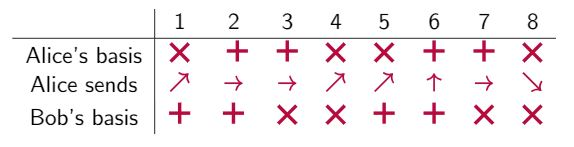
\includegraphics[scale=0.8]{bb84_q1}\]
    Calculate Alice and Bob's shared key based on the BB84 protocol described in class.
    \item \[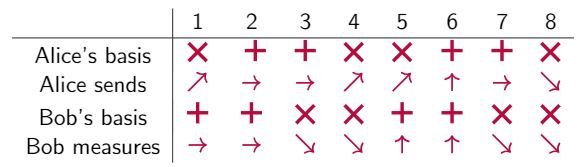
\includegraphics[scale=0.8]{bb84_q2}\]
    Now consider the same table with one additional row, Bob's measurements. Is Eve present? Which measurement gives her away and why?
    \item What is the minimum number of measurements Alice and Bob must publish in order to be at least 90\% confident Eve is not present?
    \item Suppose you and your friend Bob are trying to decide between using the E91 and BB84 protocols? What factors should you take into account? When would you prefer one protocol over the other?
    \item What is the primary property of quantum mechanics that enables the BB84 protocol?
    \item What is the primary property of quantum mechanics that enables the E91 protocol?
    \item Consider a variation on the BB84 protocol. In this protocol, Alice only has two possible states to send to Bob (as opposed to 4 in BB84). Alice will either send $\uparrow$ or $\nearrow$ to Bob. Bob will measure in either the $+$ or X basis (change the X). Let's explore how Alice and Bob can generate a shared key using these constraints.
        \begin{enumerate}
            \item Say Alice sends $\uparrow$ and Bob measures in the $+$ basis. What will Bob measure?
            \item Say Alice sends $\nearrow$ and Bob measures in the X basis. What will Bob measure?
            \item Say Alice sends $\uparrow$ and Bob measures in the X basis. What will Bob measure?
            \item Say Alice sends $\nearrow$ and Bob measures in the $+$ basis. What will Bob measure?
            \item Regardless of basis, what does Bob know about the initial state Alice sent if he measures $\uparrow$ ? What if he measures $\nearrow$ ? What if he measures  $\rightarrow$ ? What if he measures $\nwarrow$ ?
            \item Describe how Alice and Bob could construct a shared key based on the above observations. You can decide which symbol corresponds to each 0 and 1. 
            \item How could Alice and Bob detect Eve?
            \item Security of this protocol question?
        \end{enumerate}
    \item E91 table question. Very similar to Q2. Is Eve present or not? Why? Ans: Eve is present because the probability of agreement is closer to 50\% than 85\% (what it should be). To-do.
    \item I will provide an (insecure) protocol. Students must identify the problem in the protocol (prblm will likely be being unable to detect Eve)
    \item Consider the BB84 protocol. Why must Alice wait until after Bob has measured all states before publishing the bases she measured in?
    \item 3 person CHSH? Not exactly sure how this would work
    \item More CHSH and MP questions
\end{enumerate}



\end{document}